% 2011 年安徽卷理科第 17 题：多面体 ABEDFC，平面 ABED ⊥ 平面 ACFD，O 在线段 AD 上，
%   OA=1，OD=2，△OAB、△OAC、△ODE、△ODF 均为正三角形。
% 来源 PDF：普通高考/2011/2011安徽理.pdf，SHA-256 83dabf28711e3020c00f9fc73f3bf7be70f65fed94ab6ad5b6a39ac840820c0f。
% 原页：第 1 页（A3 三栏）第 3 栏下部，书页码 643。
% 重绘依据：照原页——A 在左、D 在右，B 在 A 下方、E 在 D 下方，C 在 A 上方、F 在最上方偏左；
%   A、O、D 共线且在原页画作虚线；C、E、F 与 O 的连线（OC、OE、OF）在原页为虚线（被遮挡）；
%   AC、AB、BC、BE、BF、CF、EF、FD、ED 为实线，其中 BF 原页即画作实线，照录。
%   各点按原页投影位置取相对坐标，不按原页绝对比例。
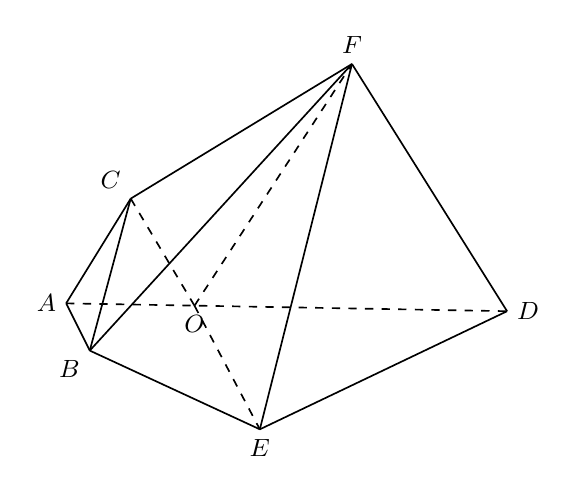
\begin{tikzpicture}[scale=1.0, >=stealth, semithick, font=\small]
  \coordinate (A) at (0,0);
  \coordinate (B) at (0.30,-0.60);
  \coordinate (C) at (0.82,1.33);
  \coordinate (O) at (1.63,-0.03);
  \coordinate (D) at (5.60,-0.10);
  \coordinate (E) at (2.46,-1.60);
  \coordinate (F) at (3.63,3.04);
  % 被遮挡的线
  \draw[dashed] (A) -- (D);
  \draw[dashed] (O) -- (C);
  \draw[dashed] (O) -- (E);
  \draw[dashed] (O) -- (F);
  % 可见的棱
  \draw (A) -- (C);
  \draw (A) -- (B);
  \draw (C) -- (B);
  \draw (B) -- (F);
  \draw (B) -- (E);
  \draw (C) -- (F);
  \draw (E) -- (F);
  \draw (F) -- (D);
  \draw (E) -- (D);
  % 顶点标注
  \node[left] at (A) {$A$};
  \node[below left] at (B) {$B$};
  \node[above left] at (C) {$C$};
  \node[below] at (O) {$O$};
  \node[right] at (D) {$D$};
  \node[below] at (E) {$E$};
  \node[above] at (F) {$F$};
\end{tikzpicture}
